\section{Algorithm progression}
\begin{frame}
	\frametitle{Algorithm progression}     
%\begin{algorithm}[H]
                                 %\SetLine
%        \SetAlgoLined
%            Initialisation\;
%            \While(The graph is not covered by the partition) {
%                auxiliaryVertices = getAuxiliaryVertices(rootIndex)\;
%                unknownVertices = auxiliary Vertices That Never Were In A Tree\;
%                knownVertices = auxiliary Vertices $\backslash$ unknownVertices\;
%                \eIf {!unknownVertices$\neq \emptyset$}{
%                      addNeededVertices(unknownVertices, rootIndex)\;
%                     }
%                     {
%                      tryVerticesSwap(knownVertices, rootIndex)\;
%                      }                              
%                     
%                        rootIndex = (rootIndex + 1) % k\;
%                }
%\end{algorithm}
%\visible <1>
%\visible <2>
%\visible <3>

%\end{frame}
%\begin{frame}
 \begin{figure}[H]
 \frametitle{}
	\begin{center}
	  % Vertices
\SetVertexNormal[MinSize=25pt,LineColor=violet,LineWidth=3pt]%V2
\Vertex[x= 2,y=0]{a}
\SetVertexNormal[MinSize=25pt,LineColor=orange,LineWidth=3pt]%V1
\Vertex[x= 6,y=2]{e}
\Vertex[x= 8,y=0]{f}
\Vertex[x= 8,y=4]{g}
\Vertex[x=10,y=2]{h}
\SetVertexNormal[MinSize=25pt,LineColor=black,LineWidth=3pt]%Vfree
\Vertex[x= 2,y=4]{b}
\Vertex[x= 4,y=2]{c}
\Vertex[x= 0,y=2]{d}
\Vertex[x=14,y=0]{i}
\Vertex[x=14,y=4]{j}
\Vertex[x=12,y=2]{k}
\Vertex[x=16,y=2]{l}
%Cliques
\Edge[lw=1pt,color=black](a)(b)%Efree
\Edge[lw=1pt,color=black](a)(c)%Efree
\Edge[lw=1pt,color=black](a)(d)%Efree
\Edge[lw=1pt,color=black](b)(c)%Efree
\Edge[lw=1pt,color=black](b)(d)%Efree
\Edge[lw=1pt,color=black](c)(d)%Efree
\Edge[lw=3pt,color=orange](e)(f)%E1
\Edge[lw=3pt,color=orange](e)(g)%E1
\Edge[lw=3pt,color=orange](e)(h)%E1
\Edge[lw=1pt,color=black](f)(g)%Efree
\Edge[lw=1pt,color=black](f)(h)%Efree
\Edge[lw=1pt,color=black](g)(h)%Efree
\Edge[lw=1pt,color=black](i)(j)%Efree
\Edge[lw=1pt,color=black](i)(k)%Efree
\Edge[lw=1pt,color=black](i)(l)%Efree
\Edge[lw=1pt,color=black](j)(k)%Efree
\Edge[lw=1pt,color=black](j)(l)%Efree
\Edge[lw=1pt,color=black](k)(l)%Efree
%Cliques Connection
\Edge[lw=1pt,color=black](a)(f)%Efree
\Edge[lw=1pt,color=black](b)(g)%Efree
\Edge[lw=1pt,color=black](f)(i)%Efree
\Edge[lw=1pt,color=black](g)(j)%Efree

	\end{center}
	\caption{step1 of the 3-connected graph partitioning: tree expansion}
      \end{figure}
\end{frame}

\begin{frame}
 \begin{figure}[H]
 \frametitle{}
	\begin{center}
	  % Vertices
\Vertex[x=7,y=5]{a} 
\Vertex[x=5,y=7]{b}
\Vertex[x=7,y=9]{c}
\Vertex[x=9,y=7]{d} 
\Vertex[x=0,y=2]{e}
\Vertex[x=2,y=4]{f}
\Vertex[x=4,y=2]{g}
\Vertex[x=2,y=0]{h}
\Vertex[x=10,y=2]{i}
\Vertex[x=12,y=4]{j}
\Vertex[x=14,y=2]{k}
\Vertex[x=12,y=0]{l}
%Cliques
\Edge[lw=3pt](a)(b)
\Edge[lw=3pt](a)(c)
\Edge[lw=3pt](a)(d)
\Edge[lw=1pt](b)(c)
\Edge[lw=1pt](b)(d)
\Edge[lw=1pt](c)(d)
\Edge[lw=3pt](e)(f)
\Edge[lw=3pt](e)(g)
\Edge[lw=3pt](e)(h)
\Edge[lw=1pt](f)(g)
\Edge[lw=1pt](f)(h)
\Edge[lw=1pt](g)(h)
\Edge[lw=1pt](i)(j)
\Edge[lw=1pt](i)(k)
\Edge[lw=1pt](i)(l)
\Edge[lw=1pt](j)(k)
\Edge[lw=1pt](j)(l)
\Edge[lw=1pt](k)(l)
%Cliques Connection
\Edge[lw=1pt](a)(f)
\Edge[lw=1pt](b)(g)
\Edge[lw=1pt](f)(i)
\Edge[lw=1pt](g)(j)

	\end{center}
	\caption{step2 of the 3-connected graph partitioning: potential swappable vertices}
      \end{figure}
\end{frame}

\begin{frame}
 \begin{figure}[H]
 \frametitle{}
	\begin{center}
	  % Vertices
\SetVertexNormal[MinSize=25pt,LineColor=violet,LineWidth=3pt]%V2
\Vertex[x= 2,y=0]{a} 
\Vertex[x= 2,y=4]{b}
\Vertex[x= 4,y=2]{c}
\Vertex[x= 0,y=2]{d}
\SetVertexNormal[MinSize=25pt,LineColor=orange,LineWidth=3pt]%V1
\Vertex[x= 6,y=2]{e}
\Vertex[x= 8,y=0]{f}
\Vertex[x= 8,y=4]{g}
\Vertex[x=10,y=2]{h}
\Vertex[x=14,y=4]{j}
\SetVertexNormal[MinSize=25pt,LineColor=black,LineWidth=3pt]%Vfree
\Vertex[x=14,y=0]{i}
\Vertex[x=12,y=2]{k}
\Vertex[x=16,y=2]{l}
%Cliques
\Edge[lw=3pt,color=violet](a)(b)%E2
\Edge[lw=3pt,color=violet](a)(c)%E2
\Edge[lw=3pt,color=violet](a)(d)%E2
\Edge[lw=1pt,color=black](b)(c)%Efree
\Edge[lw=1pt,color=black](b)(d)%Efree
\Edge[lw=1pt,color=black](c)(d)%Efree
\Edge[lw=3pt,color=orange](e)(f)%E1
\Edge[lw=3pt,color=orange](e)(g)%E1
\Edge[lw=3pt,color=orange](e)(h)%E1
\Edge[lw=1pt,color=black](f)(g)%Efree
\Edge[lw=1pt,color=black](f)(h)%Efree
\Edge[lw=1pt,color=black](g)(h)%Efree
\Edge[lw=1pt,color=black](i)(j)%Efree
\Edge[lw=1pt,color=black](i)(k)%Efree
\Edge[lw=1pt,color=black](i)(l)%Efree
\Edge[lw=1pt,color=black](j)(k)%Efree
\Edge[lw=1pt,color=black](j)(l)%Efree
\Edge[lw=1pt,color=black](k)(l)%Efree
%Cliques Connection
\Edge[lw=1pt,color=black](a)(f)%Efree
\Edge[lw=1pt,color=black](b)(g)%Efree
\Edge[lw=1pt,color=black](f)(i)%Efree
\Edge[lw=3pt,color=orange](g)(j)%E1

	\end{center}
	\caption{step3 of the 3-connected graph partitioning: vertices selection}
      \end{figure}
\end{frame}

\begin{frame}
 \begin{figure}[H]
 \frametitle{}
	\begin{center}
	  % Vertices
\SetVertexNormal[MinSize=25pt,LineColor=violet,LineWidth=3pt]%V2
\Vertex[x=4.8,y=5  ]{a} 
\Vertex[x=3.2,y=8.2]{b}
\Vertex[x=4.8,y=7  ]{c}
\Vertex[x=6.4,y=8.2]{d}
\Vertex[x=3.2,y=0  ]{f} 
\SetVertexNormal[MinSize=25pt,LineColor=orange,LineWidth=3pt]%V1
\Vertex[x=0  ,y=0  ]{e}
\Vertex[x=1.6,y=3.2]{g}
\Vertex[x=1.6,y=1.2]{h}
\Vertex[x=8  ,y=3.2]{j}
\SetVertexNormal[MinSize=25pt,LineColor=black,LineWidth=1pt]%Vfree
\Vertex[x=6.4,y=0  ]{i}
\Vertex[x=9.6,y=0  ]{k}
\Vertex[x=8  ,y=1.2]{l}
%Cliques
\Edge[lw=3pt,color=violet](a)(b)%E2
\Edge[lw=3pt,color=violet](a)(c)%E2
\Edge[lw=3pt,color=violet](a)(d)%E2
\Edge[lw=1pt,color=black](b)(c)%Efree
\Edge[lw=1pt,color=black](b)(d)%Efree
\Edge[lw=1pt,color=black](c)(d)%Efree
\Edge[lw=1pt,color=black](e)(f)%Efree
\Edge[lw=3pt,color=orange](e)(g)%E1
\Edge[lw=3pt,color=orange](e)(h)%E1
\Edge[lw=1pt,color=black](f)(g)%Efree
\Edge[lw=1pt,color=black](f)(h)%Efree
\Edge[lw=1pt,color=black](g)(h)%Efree
\Edge[lw=1pt,color=black](i)(j)%Efree
\Edge[lw=1pt,color=black](i)(k)%Efree
\Edge[lw=1pt,color=black](i)(l)%Efree
\Edge[lw=1pt,color=black](j)(k)%Efree
\Edge[lw=1pt,color=black](j)(l)%Efree
\Edge[lw=1pt,color=black](k)(l)%Efree
%Cliques Connection
\Edge[lw=3pt,color=violet](a)(f)%E2
\Edge[lw=1pt,color=black](b)(g)%Efree
\Edge[lw=1pt,color=black](f)(i)%Efree
\Edge[lw=3pt,color=orange](g)(j)%E1

	\end{center}
	\caption{step4 of the 3-connected graph partitioning: vertices swapping}
      \end{figure}
\end{frame}

\begin{frame}
 \begin{figure}[H]
 \frametitle{}
	\begin{center}
	  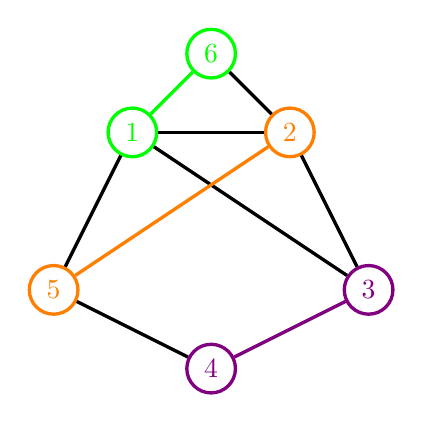
\begin{tikzpicture}
  \node[draw,circle, very thick, color=green] (A) at (1,3) {1};
  \node[draw,circle, very thick, color=orange] (B) at (3,3) {2};
  \node[draw,circle, very thick, color=violet] (C) at (4,1) {3};
  \node[draw,circle, very thick, color=violet] (D) at (2,0) {4};
  \node[draw,circle, very thick, color=orange] (E) at (0,1) {5};
  \node[draw,circle, very thick, color=green] (F) at (2,4) {6};
  \draw[very thick] (A) -- (B);
  \draw[very thick] (B) -- (C);
  \draw[very thick, color=violet] (C) -- (D);
  \draw[very thick] (D) -- (E);
  \draw[very thick] (A) -- (C);
  \draw[very thick, color=orange] (B) -- (E);
  \draw[very thick, color=green] (A) -- (F);
  \draw[very thick] (B) -- (F);
  \draw[very thick] (A) -- (E);
\end{tikzpicture}


	\end{center}
	\caption{progression toward the solution of the 3-connected graph partitioning}
      \end{figure}
\end{frame}
